% !TEX root = ../disertace.tex
%!TEX encoding = UTF-8 Unicode

\chapter{Annotation}
\label{sec:annot}

\section{Annotation – JLRE}
\label{sec:annot:jlre}

PDT 2.0 uses PML~\citep{pajas:2005}, which is an application of XML that utilizes a stand-off annotation scheme. We have extended the PDT-PML with a new schema for so-called s-files. We use these files to store all of our annotation without altering the PDT itself.
These s-files are very simple: basically each of them corresponds to one file of PDT and consists of a list of s-nodes. Each s-node corresponds to an occurrence of a MWE and is composed of a link to an entry in SemLex and a list of identifiers of t-nodes that correspond to this \mbox{s-node}. Figure~\ref{fig:s-layer} shows a relation of s-layer to PDT layers and SemLex.\footnote{Although we have created the PML schema of s-layer primarily for annotations of MWEs, we made it quite generic. It can be utilized for any treebank annotations that use a large lexicon. For instance one s-file can contain multiple annotations of valency referencing to different valency dictionaries. This generic nature of s-layer is the reason why it allows references to morphological, analytical or tectogrammatical layer of PDT, even though in our current project we only need the references to t-layer.}
%\colorbox{yellow}{TODO: odkaz na užití v anotacích podle CWN.}}.
\begin{figure}[htbp]
   \centering
   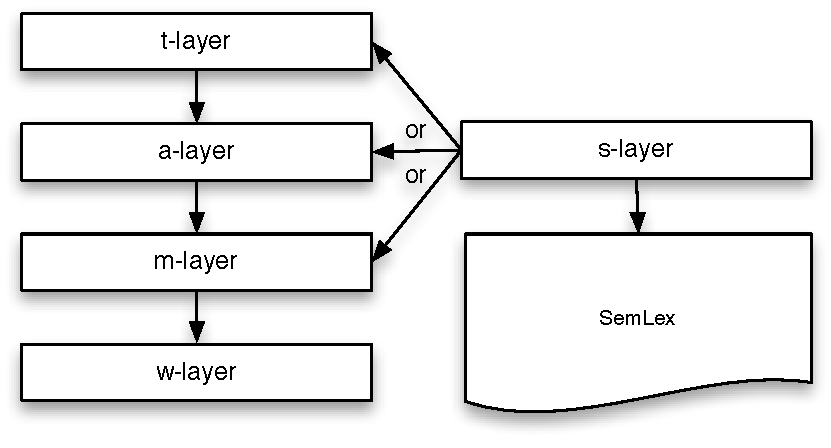
\includegraphics[scale=.5]{images/layers-with-s-layer.pdf} % requires the graphicx package
   \caption{Relation of s-layer to PDT and SemLex}
    \label{fig:s-layer}
\end{figure}


Our annotation program reads in a tectogrammatical representation (t-file) and calls TrEd \citep{pajas:tred} to generate plain text. This plain text (still linked to the tectogrammatical representation) is presented to the annotator. While the annotator marks MWEs already present in SemLex or adds new MWEs into SemLex, tree representations of these MWEs extracted from underlying t-trees are added into their SemLex entries via TrEd scripts. 

%These tree representations are quite simple: for each node in a MWE we only record its t-lemma and its father's ID.


%%%%%
\section{Pre-annotation}
\label{sec:annot:pre}
Because MWEs tend to occur repeatedly in a text, we have decided to test pre-annotation both for speed improvement and for improving the consistency of annotations. 
%We work o
On the assumption that \emph{all occurrences of a MWE share the same tree structure}, while there are no restrictions on the surface word order other than those imposed by the tree structure itself
%
% pre-annotation types
%W
we have decided to employ four types of pre-annotation:

\begin{asparaenum}[A)]
\item \label{pre-hnatkova}External pre-annotation provided by our colleague (see~\citealp{hnatkova:2002}). With each MWE a set of rules is associated that limits possible forms and surface word order of parts of a MWE. This approach was devised for corpora that are not syntactically annotated and is very time consuming.
\item \label{pre-static}Our one-time pre-annotation with those MWEs from SemLex that have been previously used in annotation, and thus have a tree structure as a part of their entry.
\item \label{pre-on-load}Dynamic pre-annotation as in \ref{pre-static}, only with the SemLex entries that have been recently added by the annotator. 
\item \label{pre-on-annot}When an annotator tags an occurrence of a MWE in the text, other occurrences of this MWE in the article are identified automatically.%
%
\footnote{This is exactly what happens:
\begin{inparaenum}[1)]
\item Tree structure of the selected MWE is identified via TrEd
\item The tree structure is added to the lexeme's entry in SemLex
\item All the sentences in the given file are searched for the same MWE using its tree structure (via TrEd)
\item Other occurrences returned by TrEd are tagged with this MWE's ID, but these occurrences receive an attribute ``auto'', which identifies them (both in the s-files and visually in the annotation tool) as annotated automatically.
\end{inparaenum}
} % end footonote
\end{asparaenum}

Pre-annotation (\ref{pre-hnatkova})~was executed once for all of the PDT. (\ref{pre-static})~is performed each time we merge MWEs added by annotators into the main SemLex. We carry out this annotation in one batch for all PDT files remaining to annotate. (\ref{pre-on-load})~is done for each file while it is being opened in the annotation environment. 
(\ref{pre-on-annot})~happens each time the annotator adds a new MWE into SemLex and uses it to annotate an occurrence in the text. In subsequent files instances of this MWE are already annotated in step (\ref{pre-on-load}), and later even in (\ref{pre-static}).
%, when the lexia (lexicon entry) is merged into the main SemLex. 
 
% PRO FUTURA
%We have currently performed double blind annotation of a part of data without pre-annotation (\ref{pre-static}) and (\ref{pre-on-load}). We also have smaller samples annotated without any pre-annotation and only with pre-annotation (\ref{pre-hnatkova}). Analysis of this data is necessary  to show that our assumption is correct and all the occurrences of a lexia share the same tree structure. Then we can safely add remaining pre-annotation steps. Provided the inter-annotator agreement is good enough we can also stop our current (rather expensive and time consuming) practice of double annotation of each file and comparing the annotations. 

After the pilot annotation without pre-annotation (\ref{pre-on-annot})  we have compared instances of the same tags and found that 10.5\% of repeated MWEs happened to have two different tree representations. Below we analyse several most important sources of these inconsistent t-trees and possible improvements:
\begin{itemize}
%
\item \emph{Occasional lemmatisation errors.} They are not very frequent, but there is no efficient way to find and correct them before the annotations. So there is not much we can do but it is not very important. Our annotations can however serve as a source for automatic corrections.
	\begin{itemize}
	\item \textit{jižní Korea {\rm vs.} Jižní Korea} (southern vs. South Korea)
	\end{itemize}
% chyba anotatora (neoznaci v LexSemAnnu slovo)
\item \emph{Annotator's mistake (not marking correct words).} When an annotator makes an error while marking a first occurrence of a MWE, the tree representation that gets stored in SemLex is incorrect. As a result, pre-annotation gives false positives or fails to work. 

It is therefore necessary to allow annotators to correct the tree structure of a SemLex entry, i.e. extend functionality of the annotation tool. Once all the types of pre-annotation are employed, this error can happen only once, because all the following occurrences of a MWE are pre-annotated automatically. We are currently working on these improvements.
%
\item \emph{Gender opposites, diminutives and augmentatives.} These are currently represented by variations of t-lemma. 
We believe that they should be represented by attributes of t-nodes %, which would explicate information that is now given only implicitly. 
that could be roughly equivalent to some of the lexical functions in the Meaning-text theory (see \cite{melcuk:1992}).
This should be tackled in some future version of PDT. Once resolved it would allow us to identify following (and many similar) cases automatically. 
	\begin{itemize}
	\item \textit{obchodní ředitel {\rm vs.} obchodní ředitelka} \\(lit.: managing director-man vs. m. director-woman)
	\item \textit{rodinný dům {\rm vs.} rodinný domek} \\(lit.: family house vs. family little-house; but the diminutive \emph{domek} means basically “family house”)
	\end{itemize}
%
Currently we annotate these cases with the same MWE, but all the instances with the derived variants of t-lemma (like \emph{ředitelka } or \emph{domek} must be identified manually (see Section~\ref{sec:pre}). We plan to try automatic identification of some diminutives and gender opposites derived by most common patterns.

%
\item \emph{Newly established t-nodes corresponding to elided parts of MWEs in coordinations.} Since t-layer contains many newly established t-nodes, many of whom cannot be lexicalised, our original decision was to hide all of these nodes from annotators and generate for them pure surface sentence. This decision resulted however in the current situation, when some MWEs in coordinations cannot be correctly annotated. 
%It is necessary to elide common part of coordinated multiword lexeme. 
For instance \emph{První a druhá světová válka} (First and Second World War) is a coordination of two multiword lexemes. A tectogrammatical tree that includes it does have newly established t-nodes for “world” and “war” of the first lexeme but they are elided in the surface sentence. 

After analysing annotated examples like the one above we have decided to generate surface words from some of the newly established t-nodes in order to allow correct annotation of all the MWEs. These ``added'' words will be displayed in grey and while some morphological forms of these words may be incorrect, we believe they will serve their purpose.

% the first lexeme cannot be identified automatically. In this and other similar cases t-nodes for elided parts of multiword lexemes should have been part of PDT, in our opinion. Given that our goal is to have one t-node for each lexia, however, we believe it would not be efficient to invest substantial amount of manual work into adding these elided t-nodes now only to eliminate them more efficiently in near future. We can just as well leave it to our annotators to identify these instances of MWEs (it is as common for NEs, as it is for lexias) manually.
%
%\item \emph{Bridging anaphora} e.g. Ceska narodni banka <- banka \\
%Since in the context the second expression stands for the first only with some words ellided, our annotators were instructed to annotate it as an instance of the lexia \emph{Česká národní banka}. 

%This problem could be solved by annotations of coreference. If the coreference between nominal expressions was present in the PDT 2.0, our annotators would simply mark the first occurence and all the anaphoric expressions would be marked automatically. 
\end{itemize}

% spojit s 'itemize' vyse!
% because these cases are caused by ellipses, variations in lexical form such as diminutives etc., or wrong lemmatisation, rather than inconsistencies in the tree structure. These cases show us some problematic issues in PDT 2.0, for instance:
%\begin{itemize}
%\item \textit{jižní Korea {\rm vs.} Jižní Korea} \\(southern vs. South Korea) -- wrong lemmatisation
%\item \textit{obchodní ředitel {\rm vs.} obchodní ředitelka} \\(lit. managing director-man vs. m. director-woman) -- in future these should have one t-lemma. Morphological gender should be specified by an attribute of a t-node.
%\end{itemize}

Up to now we have not found any MWE such that its structure cannot be represented by a single tectogrammatical tree. 1.1\% of all occurrences were not connected graphs, but this happened due to errors in data and to our incorrect handling of coordinations with newly established t-nodes (see above). This corroborates our assumption that (disregarding errors) all occurrences of a MWE share the same tree structure. As a result, we started storing the tree structures in the SemLex entries and employ them in pre-annotation (\ref{pre-on-annot}). This also allows us to use pre-annotations (\ref{pre-static}) and (\ref{pre-on-load}), but we have decided not to use them at the moment, in order to be able to evaluate each pre-annotation step separately. Thus the following section reports on the experiments that employ pre-annotations (\ref{pre-hnatkova}) and (\ref{pre-on-annot}).


%%%%%
\section{Analysis of Annotations – JLRE}
\label{sec:annot:analysis}
Two annotators have started to use (and test) the tool we have developed.
They both have got the same texts. The text is generated from the t-trees and presented as a plain text with pre-annotated words mark\-ed by colour labels. Annotators add their tags in the form of different colour labels and they can delete the pre-annotated tags. 
In this experiment the data consists of approx. 310,000 tokens, which correspond to 250,000 t-nodes.
Both annotators have marked about 37,000 t-nodes ($\approx$ 15\%) as parts of MWEs and grouped them into 17,000 MWEs. So the average length of a MWE is 2.2 t-nodes.
% Annotator $A$ %Vimmrova
% has grouped them into 7,263 MWEs and annotator $B$ %Sidak
% into 6,888. So the average length of a MWE is 2.2 t-nodes.

The ratio of general named entities versus SemLex entries was 50:50 for annotator $A$ and 52:48 in the case of annotator $B$. Annotator $A$ used SemLex more frequently (than she used named entities and also than annotator $B$ used SemLex), but did not utilize as many lexicon items as annotator $B$.
% Annotator $B$ used 10\% more lexias than annotator $A$ (3,279 and 3,677), while they both used almost the same number of NEs.
This and some other comparison is given in Table~\ref{tab:anot}.


\begin{table}[h]
\centering
\begin{tabular}{l|r|r}
type of MWE&$A$&$B$\\
\cline{1-3}
SemLex entries&8,447&8,312\\
 - different items&3,844&4,089\\
Named Entities&8,435&8,903\\
 - person/animal&2,797&2,811\\
 - institution&1,702&2,047\\
 - number&1,343&1,053\\
 - object&1,129&888\\
\end{tabular}
\caption{Annotated instances \newline of significant types of MWEs}
\label{tab:anot}
\end{table}

Both annotators also needed to add missing entries to the originally compiled SemLex or to edit existing entries. Annotator $A$ added 1,361 entries while annotator $B$ added 2,302. They modified 1,307 and 2,127 existing entries, respectively.


\subsection{Inter-annotator Agreement – JLRE}
\label{agreement}

In this section our primary goal is to assess whether with our current methodology we produce a reliable annotation of MWEs. To that end we measure the amount of inter-annotator agreement that is above chance. Our attempt exploits {\it weighted kappa measure} $\kappa_w$ \cite{cohen:1968}.

The reason for using a weighted measure is essential for our task: we do not know which parts of sentences are MWEs and which are not. Therefore annotators work with all words and even if they do not agree on the type of a particular MWE, it is still an agreement on the fact that this t-node is a part of some MWE and thus should be tagged. This means we have to allow for partial agreement on a tag.

There are, however, a few sources of complications in measuring agreement of our task even by $\kappa_w$:
\begin{itemize}
	\item % castecne pruniky tagu
	Each tag of a MWE identifies a subtree of a tectogrammatical tree (represented on the surface by a set of marked words). This allows for partial agreement of tags at the beginning, at the end, but also in the middle of a surface interval (in a sentence). Instead, standard measures like $\kappa$ assumes fixed, bounded items, which are assigned some categories.
	\item % nejasny pocet tagu
	There is no clear upper bound as to how many (and how long) MWEs there are in texts. Cohen's $\kappa_w$ counts agreement on known items and these are the same for both annotators. On the other hand, we want to somehow count agreement on the fact, that given word is not a part of MWE.
% [to sem nepatri, leda pouzit jinde] Since the disagreement in $\kappa$ is substracted from one and one is unreachable,\footnote{Let say that both annotators say some word is not part of a MWE, we treat it like an agreement..........} we should use another upper bound.
	\item 
	There is not a clear and simple way to estimate the amount of agreement by chance, because it must include the partial agreements mentioned above.
\end{itemize}

Since we want to keep our agreement calculation as simple as possible but we also need to take into account the issues above, we have decided (as mentioned above) to start from $\kappa_w$ as defined in \cite{artstein:2007}: $\kappa_w = 1 - \frac{D_o}{D_e} = \frac{A_o - A_e}{1 - A_e}$ (explanation in Equation \ref{ourkappa}) and to make a few adjustments to allow for an agreement on non-annotation and an estimated upper bound. We explain these adjustments in following paragraphs.


Because we do not know how many MWEs there are in our texts, we need to \textit{calculate the agreement over all t-nodes}, rather than just the \mbox{t-nodes} that ``should be annotated''. This also means that the theoretical maximal agreement (upper bound) $U$ cannot be 1. If it was 1, it would be saying that all nodes are part of MWEs. 

Since we know that $U < 1$ but we do not know its exact value, we use the \textit{estimated upper bound} $\widehat{U}$ (see Equation \ref{eq-upper-bound}). Because we calculate $\widehat{U}$ over all t-nodes, we need to account not only for agreement on tagging a t-node, but also for agreement on a t-node not being a part of a MWE, i.e. not tagged at all. 
%
%\footnote{If we did not do this, there would be no difference between t-nodes, that were not tagged (annotators agreed they are not a part of a MWE) and the t-nodes that one annotator tagged and the other did not (i.e. they disagreed).}
%
This allows us to positively discriminate the cases where annotators agree that a t-node is not a part of a MWE from the cases where one annotator annotates a t-node and the other one does not, which is evidently worse.

%\newpage
If $N$ is the number of all t-nodes in our data and $n_{A \cup B}$ is the number of t-nodes annotated by at least one annotator, then we estimate $\widehat{U}$ as follows:
\begin{equation}
\label{eq-upper-bound}
\widehat{U} = \frac{n_{A \cup B}}{N} + 0.051 \cdot \frac{N - n_{A \cup B}}{N}= 0.213.
\end{equation}

The weight $0.051$ used for scoring the t-nodes that were not annotated is explained below ($c=4$). Because $\widehat{U}$ includes all the disagreements of the annotators, we believe that the real upper bound $U$ lies somewhat below it and the agreement value 0.213 is not something that should (or could) be achieved. It is however based on the assumption that the data we have not yet seen have similar proportion of MWEs as the data we have used for the upper bound estimate.

To account for partial agreement we divide the t-nodes into 5 classes $c$ and assign each class a weight $w_c$ as follows: 

\begin{enumerate}[$c=1$]
\item
If the annotators agree on the exact tag from SemLex, we get maximum information: $w_1 = 1$.
\item
If they agree that the t-node is a part of a NE or they agree that it is a part of some entry from SemLex, but they do not agree which NE or which entry, we estimate we get about a half of the information compared to when $c=1$: $w_2 = 0.5$.
\item
If they agree that the t-node is a part of a MWE, but disagree whether a NE or an entry from SemLex, it is again half the information compared to when $c=2$, so $w_3 = 0.25$.
\item
If they agree that the t-node is not a part of a MWE, $w_4 = 0.051$. This low value of $w$ accounts for frequency of t-nodes that are not a part of a MWE, as estimated from data: Agreement on not annotating provides the same amount of information as agreement on annotating, but we have to take into account higher frequency of t-nodes that are not annotated: 
  \[  w_4 = w_3 \cdot \frac{\sum annotated}{\sum not\ annotated} = 0.25 \cdot \frac{42779}{208437} \approx 0.051. \]
We can see that two ideal annotators who agree on all their assignments could not reach high agreement measure, since they naturally leave some t-nodes without an annotation and even if they are the same t-nodes for both of them, this agreement is weighted by $w_4$. Now we can look back at Equation \ref{eq-upper-bound} and see that $\widehat{U}$ is exactly the agreement which two ideal annotators reach.

It should be explained why we do not need to corrected upper bound when working with weighted measures like $\kappa_w$.
There are weights for some types of disagreement in $\kappa_w$ to distinguish ``better'' disagreement from ``worse'' one. But it is still a disagreement and annotators could agree completely. While in our task this class $c=4$ represents agreement of its kind. The reason why we do not count it as an agreement is the biased resulting measure, if we do so.%
\footnote{%
We have also measured standard $\kappa$ without weights. All partial disagreements were treated as full disagreements. In $\kappa_1$ we counted every non-annotated t-node as a disagreement, too; in $\kappa_2$ we think of non-annotation as a new category (with common agreement). And the difference is quite clear ($\kappa_1 = 0.04$ and $\kappa_2 = 0.68$) although $\kappa$ is an agreement above chance and the expected agreement by chancewas also different in $\kappa_1$ and $\kappa_2$.}
The lesser they annotate the higher the agreement would be (with the extreme case of $\kappa = 1$ when they annotate nothing).
 
\item
If the annotators do not agree whether to annotate a t-node or not, $w_5 = 0$. 
\end{enumerate}

%\newpage 
The numbers of t-nodes $n_c$ and weights $w$ per class $c$ are given in Table~\ref{tab-agreement}.

\begin{table}[H]
\begin{center}
 \begin{tabular}{l|c|c|c|c|c}

&\multicolumn{4}{c|}{Agreement} & Disagreement\\
\cline{2-6}
&\multicolumn{3}{c|}{Annotated} & Not annot. &  \\
\cline{2-5}
&\multicolumn{2}{c|}{Agr. on NE / SL entry} &&&\\
\cline{2-3}
&Full agr. & Disagr. &&&\\
\cline{1-6}
class $c$& 1 & 2 & 3 & 4 & 5\\
\cline{1-6}
\# of t-nodes $n$& 24,386 & 6,355 & 1,399 & 208,437 & 10,639\\
\cline{1-6}
weight $w$ & 1 & 0.5 & 0.25 & 0.051 & 0 \\
\cline{1-6}
$w_c n_c$ & 24,386 & 3,178 & 350 & 10,695 & 0\\
\end{tabular}
\end{center}
\caption{The agreement per class and the associated weights}
\label{tab-agreement}
\end{table}


Now that we have estimated the upper bound of agreement $\widehat{U}$ and the weights $w$ for all t-nodes we can calculate our version of weighted~$\kappa_w$:

\begin{equation}
\label{ourkappa}
\kappa_w^U = \frac{A_o - A_e}{\widehat{U} - A_e} =
             \frac{D_e - D_o}{\widehat{U} - 1 + D_e}\ .
\end{equation}

$A_o$ is the observed agreement of annotators and $A_e$ is the agreement expected by chance (which is similar to a baseline). $\kappa_w^U$ is thus a simple ratio of our observed agreement above chance and maximum agreement above chance. In equivalent (and often used) definition, $D_o$ and $D_e$ are observed and expected disagreements.

Weights $w$ come into account in calculation of $A_o$ and $A_e$.

We calculate $A_o$ by multiplying the number of t-nodes in each category $c$ by that category's weight $w_c$ (see Table \ref{tab-agreement}), summing these five weighted sums and dividing this sum of all the observed agreement in the data by the total number of t-nodes:
%\begin{align*}
\[	A_o = \frac{1}{N} \sum_{c =1}^{5} w_c n_c = \\
%\frac{1}{100556} ((6908+3619)\cdot1 + (437+1928)\cdot0.5 + 389\cdot0.25 + 83287\cdot0.052 + 3988\cdot0) =
	 \frac{1}{251216} (24386 + 3178 + 350 + 10695 + 0) \doteq 0.154.
	\]
%\end{align*}

$A_e$ is the probability of agreement expected by chance over all t-nodes. This means it is the sum of the weighted probabilities of all the combinations of all the tags that can be obtained by a pair of annotators. Every possible combination of tags (including not tagging a t-node) falls into one of the categories $c$ and thus gets the appropriate weight $w$. (Let us say a combination of tags $i$ and $j$ has a probability $p_{ij}$ and is weighted by $w_{ij}$.)
%\begin{compactitem}
%\item
%If there is an agreement on a tag, we are in $c_1$ (and $w_1 = 1$).
%\item
%When there are two tags but not identical, we are in $c_2$ or $c_3$. This depends on whether there is an agreement on choosing the same type of a SemLex entry: NE or lexia.
%\item
%An agreement on not annotating is in class $c_4$.
%\item
%A disagreement on whether to annotate falls into the class $c_5$.
%\end{compactitem}
%

We estimated these probabilities from annotated data
\[
A_e = \sum_i^{SemLex} \sum_j^{SemLex}
	\frac{n_{q_iA}}{N_A} \frac{n_{q_jB}}{N_B} w_{ij} \approx 0.046\ ,
\]
where $n_{q_iA}$ is the number of lexicon entry $q_i$ in annotated data from annotator $A$ and $N_A$ is the amount of t-nodes given to annotator $A$. Here, the non-annotation is treated like any other label assigned to a t-node.

The resulting $\kappa_w^U$ is then
%\[\pi_w = \frac{A_o - A_e}{\widehat{U} - A_e} = \frac{0.160 - 0.047}{0.215 - 0.047} = 0.676.\]
\[\kappa_w^U = \frac{A_o - A_e}{\widehat{U} - A_e} = \frac{0.154 - 0.046}{0.213 - 0.046} \doteq 0.644.\]

We introduced improved $\kappa_w^U$ measure, which is weighted kappa with the upper bound moved from the value 1. We also inspected other measures like simple $\kappa$ (results differ according to the treatment of non-annotated t-nodes: $\kappa_1 = 0.04$ and $\kappa_2 = 0.68$), or weighted variant of $\pi$ with no respect for individual coder distributions (but with results almost exactly the same as $\kappa$: $\pi_w = 0.644$).

When we analyse disagreement and partial agreement we find that most cases have to do with SemLex entries rather than NEs. This is mostly due to the deficiencies of the dictionary and its size (annotators could not explore each of almost 30,000 of SemLex entries). Our current methodology, which relies too much on searching the SemLex, is also to blame. This should, however, improve by employing pre-annotations (\ref{pre-static}) and (\ref{pre-on-load}). 

%\begin{compactitem}
%\item 
One more reason for disagreement consists in the fact that there are cases for which non-trivial knowledge of the world is needed: ``Jang Di Pertuan Agong Sultan Azlan Shah, the sultan of the state of Perak, [\kern 2pt \ldots] flew back to Perak.'' Is ``Sultan Azlan Shah'' still a part of the name or is it (or a part of it) a title?
%\item 

The last important cause of disagreement is simple: both annotators identify \emph{the same} part of text as MWE instances, but while searching the SemLex they choose different entry as the tags. This can be rectified by:
	\begin{compactitem}
		\item Removing duplicate entries from SemLex (currently there are many almost identical entries originating from Eurovoc and Czech WordNet).
		\item Imploring improved pre-annotation \ref{pre-static} and \ref{pre-on-load}, as mentioned above.
	\end{compactitem}
%\end{compactitem}
%\medskip

%We have recently begun annotations of pre-annota\-ted data (type \ref{pre-hnatkova}). If we may infer from such small data (319 lexias), this type of pre-annotation slightly helps on SemLex entries (it was the object of pre-annotation, from 34.7\% to 36.5\%) and slightly spoils the NE agreement (from 71.8\% to 67.1\%). Generally, on all lexias, it slightly improves agreement (from 58.2\% to 60.1\%). Speed improvement was quite noticeable, because vast majority of pre-annotated tags might be left untouched by annotators.


% k PI:
% nase Max. je zalozene na predpokladu, ze data budou nadale podobne a anotatori nezacnou naraz anotovat vyrazne vic. 
% Max. je stanoveno tak, ze za predpokladu vyse anotator nemuze (a ani nema) Max. dosahnout. Jelikoz jde o prunik vsech anotovanych uzlu, jsou v nem i chyby (v neshodach), ty ale kompenzuji pripadne uzly, ktere ani jeden neidentifikoval, ale meli.